\documentclass[11pt,a4paper]{article}

\usepackage[a4paper, top=18mm, bottom=18mm, left=16mm, right=18mm]{geometry}
\usepackage{tikz}
\usetikzlibrary{shapes.geometric,arrows.meta,positioning,fit,backgrounds,
                calc,decorations.pathreplacing,matrix}
\usepackage{booktabs}
\usepackage{array}
\usepackage{xcolor}
\usepackage{colortbl}
\usepackage{enumitem}
\usepackage{tabularx}
\usepackage{multicol}
\usepackage{multirow}
\usepackage{titlesec}
\usepackage{fancyhdr}
\usepackage{hyperref}
\usepackage{amsmath}
\usepackage{pifont}
\usepackage{makecell}
\usepackage{caption}

%% ── colours ────────────────────────────────────────────────────────────────
\definecolor{navy}{HTML}{1B2A4A}
\definecolor{steel}{HTML}{2E6DA4}
\definecolor{sky}{HTML}{C8DDEF}
\definecolor{teal}{HTML}{2A9D8F}
\definecolor{teallt}{HTML}{D0EEEC}
\definecolor{red}{HTML}{C0392B}
\definecolor{redlt}{HTML}{FADBD8}
\definecolor{amber}{HTML}{E67E22}
\definecolor{amberlt}{HTML}{FDEBD0}
\definecolor{grn}{HTML}{1E8449}
\definecolor{grnlt}{HTML}{D5F5E3}
\definecolor{lgray}{HTML}{F4F6F7}
\definecolor{mgray}{HTML}{BDC3C7}
\definecolor{dkgray}{HTML}{555555}
\definecolor{purp}{HTML}{6C3483}
\definecolor{purplt}{HTML}{E8DAEF}

%% ── hyperref ────────────────────────────────────────────────────────────────
\hypersetup{colorlinks,linkcolor=steel,urlcolor=teal}

%% ── page style ──────────────────────────────────────────────────────────────
\pagestyle{fancy}\fancyhf{}
\fancyhead[L]{\small\textcolor{navy}{\textbf{Arbitration Logic \& Command Selector — Deep Reference}}}
\fancyhead[R]{\small\textcolor{red}{DDR MC Core}}
\fancyfoot[C]{\small\thepage}
\renewcommand{\headrulewidth}{0.4pt}

%% ── section style ───────────────────────────────────────────────────────────
\titleformat{\section}{\large\bfseries\color{navy}}{\thesection}{0.6em}{}
  [\vspace{-4pt}\textcolor{navy}{\rule{\linewidth}{0.5pt}}]
\titleformat{\subsection}{\normalsize\bfseries\color{steel}}{\thesubsection}{0.5em}{}
\titleformat{\subsubsection}{\small\bfseries\color{teal}}{\thesubsubsection}{0.5em}{}
\titlespacing{\section}{0pt}{10pt}{4pt}
\titlespacing{\subsection}{0pt}{7pt}{2pt}
\titlespacing{\subsubsection}{0pt}{5pt}{1pt}

%% ── list style ──────────────────────────────────────────────────────────────
\setlist[itemize]{itemsep=1pt,topsep=2pt,parsep=0pt,
                  label=\textcolor{steel}{$\blacktriangleright$}}
\setlist[itemize,2]{label=\textcolor{teal}{$\circ$},leftmargin=1.5em}

%% ── table macros ────────────────────────────────────────────────────────────
\newcommand{\THead}[1]{\cellcolor{navy}\textcolor{white}{\small\textbf{#1}}}
\newcommand{\THs}[1]{\cellcolor{steel}\textcolor{white}{\small\textbf{#1}}}
\newcommand{\RA}{\rowcolor{lgray}}
\newcommand{\RB}{\rowcolor{sky!30}}
\newcommand{\cmark}{\textcolor{grn}{\ding{51}}}
\newcommand{\xmark}{\textcolor{red}{\ding{55}}}
\arrayrulecolor{mgray}

%% ── TikZ styles ─────────────────────────────────────────────────────────────
\tikzset{
  blk/.style={rectangle,rounded corners=3pt,draw=#1,fill=#1!12,
              minimum width=2.8cm,minimum height=0.7cm,
              font=\small\bfseries,align=center,text=#1,
              inner sep=4pt},
  sblk/.style={rectangle,rounded corners=2pt,draw=#1,fill=#1!10,
               minimum width=2.4cm,minimum height=0.58cm,
               font=\scriptsize,align=center,text=#1},
  submod/.style={rectangle,rounded corners=2pt,draw=steel,fill=sky!40,
                 minimum width=2.2cm,minimum height=0.55cm,
                 font=\scriptsize\bfseries,align=center,text=navy},
  pool/.style={rectangle,rounded corners=2pt,draw=teal,fill=teallt,
               minimum width=1.8cm,minimum height=0.55cm,
               font=\scriptsize,align=center,text=teal},
  st/.style={circle,draw=navy,fill=sky!50,minimum size=1.0cm,
             font=\scriptsize\bfseries,align=center,text=navy},
  arr/.style={-Stealth,thick,color=navy},
  rarr/.style={-Stealth,thick,color=red},
  tarr/.style={-Stealth,thick,color=teal},
  aarr/.style={-Stealth,thick,color=amber},
  grp/.style={rectangle,rounded corners=5pt,draw=#1!60,fill=#1!4,
              dashed,inner sep=7pt},
  lbl/.style={font=\tiny,color=dkgray},
}

\setlength{\parskip}{2pt}\setlength{\parindent}{0pt}
\captionsetup{font=small,labelfont={bf,color=navy},skip=3pt}

%%%%%%%%%%%%%%%%%%%%%%%%%%%%%%%%%%%%%%%%%%%%%%%%%%%%%%%%%%%%%%%%%%%%%%%%%%%%
\begin{document}

%% ── TITLE ───────────────────────────────────────────────────────────────────
\begin{center}
  {\LARGE\bfseries\color{navy} Arbitration Logic \& Command Selector}\\[4pt]
  {\large\color{steel} DDR Memory Controller Core — Detailed Reference}\\[2pt]
  {\small\color{dkgray}
   Covers: internals $\cdot$ data-flow $\cdot$ constraint enforcement
   $\cdot$ supported/unsupported checklist}
\end{center}
\vspace{-4pt}\hrule height 0.8pt\vspace{6pt}

%%%%%%%%%%%%%%%%%%%%%%%%%%%%%%%%%%%%%%%%%%%%%%%%%%%%%%%%%%%%%%%%%%%%%%%%%%%%
\section{System Context}
%%%%%%%%%%%%%%%%%%%%%%%%%%%%%%%%%%%%%%%%%%%%%%%%%%%%%%%%%%%%%%%%%%%%%%%%%%%%

These two blocks occupy the \textbf{decision pipeline} of the MC Core,
between the CDC crossing and the DFI interface.
They are the sole arbiters of \emph{what} goes to DRAM and \emph{when}.

\vspace{6pt}
\begin{center}
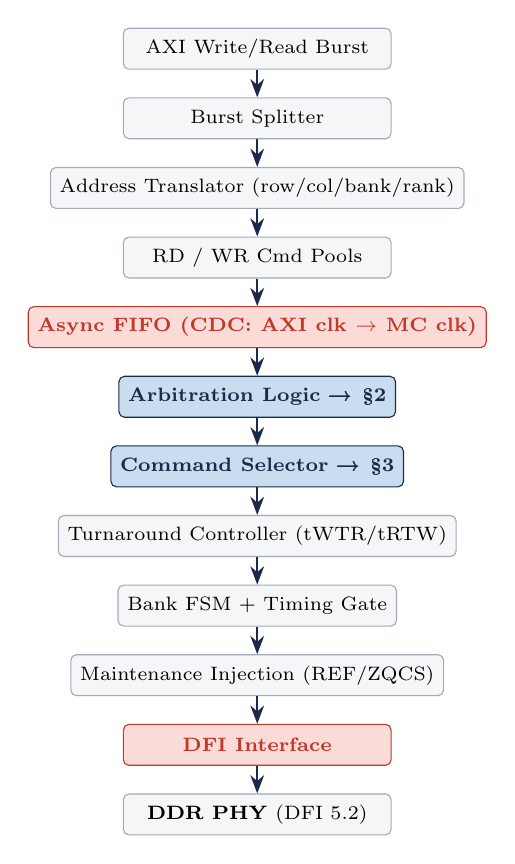
\begin{tikzpicture}[node distance=0.35cm and 0.0cm]
  \tikzset{fl/.style={rectangle,draw=navy!40,fill=lgray,rounded corners=2pt,
    minimum width=3.4cm,minimum height=0.52cm,font=\scriptsize,align=center}}
  \tikzset{hl/.style={rectangle,draw=navy,fill=sky,rounded corners=2pt,
    minimum width=3.4cm,minimum height=0.52cm,font=\scriptsize\bfseries,
    text=navy,align=center}}
  \tikzset{sep/.style={rectangle,draw=red,fill=redlt,rounded corners=2pt,
    minimum width=3.4cm,minimum height=0.52cm,font=\scriptsize\bfseries,
    text=red,align=center}}

  \node[fl]  (a1) {AXI Write/Read Burst};
  \node[fl,below=of a1] (a2) {Burst Splitter};
  \node[fl,below=of a2] (a3) {Address Translator (row/col/bank/rank)};
  \node[fl,below=of a3] (a4) {RD / WR Cmd Pools};
  \node[sep,below=of a4] (a5) {Async FIFO (CDC: AXI clk $\to$ MC clk)};
  \node[hl,below=of a5]  (a6) {\textbf{Arbitration Logic} \textrightarrow\ \S2};
  \node[hl,below=of a6]  (a7) {\textbf{Command Selector} \textrightarrow\ \S3};
  \node[fl,below=of a7]  (a8) {Turnaround Controller (tWTR/tRTW)};
  \node[fl,below=of a8]  (a9) {Bank FSM + Timing Gate};
  \node[fl,below=of a9]  (a10){Maintenance Injection (REF/ZQCS)};
  \node[sep,below=of a10](a11){DFI Interface};
  \node[fl,below=of a11] (a12){\textbf{DDR PHY} (DFI 5.2)};

  \foreach \i/\j in {a1/a2,a2/a3,a3/a4,a4/a5,a5/a6,a6/a7,
                     a7/a8,a8/a9,a9/a10,a10/a11,a11/a12}
    \draw[arr] (\i)--(\j);
\end{tikzpicture}
\end{center}

%%%%%%%%%%%%%%%%%%%%%%%%%%%%%%%%%%%%%%%%%%%%%%%%%%%%%%%%%%%%%%%%%%%%%%%%%%%%
\section{Arbitration Logic}
%%%%%%%%%%%%%%%%%%%%%%%%%%%%%%%%%%%%%%%%%%%%%%%%%%%%%%%%%%%%%%%%%%%%%%%%%%%%

\subsection{Function}

Runs every MC clock. Answers: \textbf{``which command class wins this cycle?''}
Does \emph{not} pick bank/row/col — that is Command Selector's domain.
Output: winner class + pool pointer into winning queue.

\subsection{Internal Block Diagram}

\begin{center}
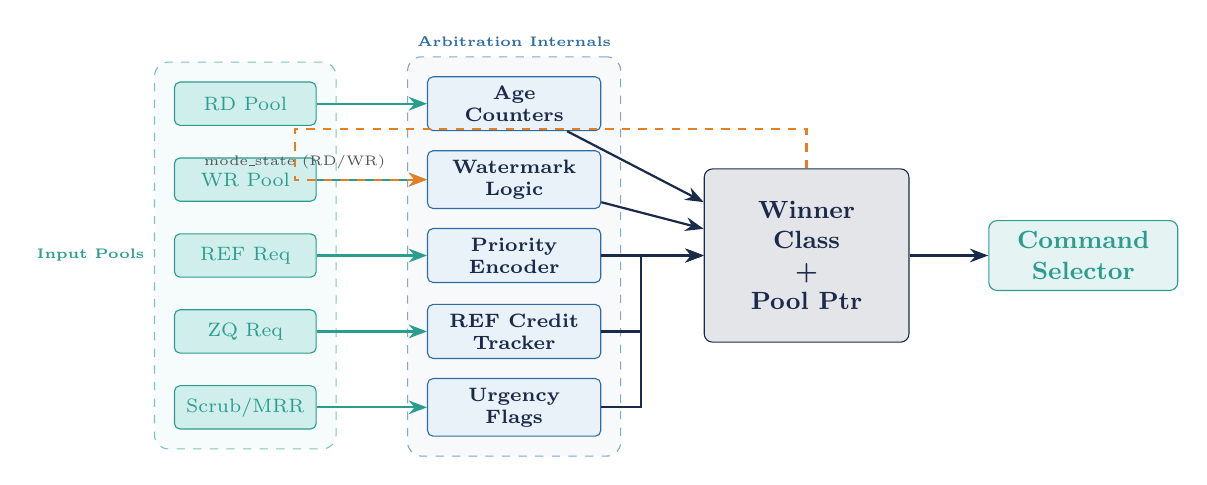
\begin{tikzpicture}[node distance=0.6cm and 1.1cm]

  %% ── input pools ──────────────────────────────────────────────────────────
  \node[pool] (rd)  {RD Pool};
  \node[pool,below=0.4cm of rd]  (wr)  {WR Pool};
  \node[pool,below=0.4cm of wr]  (ref) {REF Req};
  \node[pool,below=0.4cm of ref] (zq)  {ZQ Req};
  \node[pool,below=0.4cm of zq]  (mnt) {Scrub/MRR};

  %% ── internal submodules ──────────────────────────────────────────────────
  \node[submod,right=1.4cm of rd]   (age) {Age\\Counters};
  \node[submod,right=1.4cm of wr]   (wm)  {Watermark\\Logic};
  \node[submod,right=1.4cm of ref]  (penc){Priority\\Encoder};
  \node[submod,right=1.4cm of zq]   (cred){REF Credit\\Tracker};
  \node[submod,right=1.4cm of mnt]  (urg) {Urgency\\Flags};

  %% ── output ───────────────────────────────────────────────────────────────
  \node[blk=navy,right=1.3cm of penc,
        minimum width=2.6cm,minimum height=2.2cm]
        (out) {Winner\\Class\\+\\Pool Ptr};

  %% ── arrows inputs → submodules ───────────────────────────────────────────
  \draw[tarr] (rd)  -- (age);
  \draw[tarr] (wr)  -- (wm);
  \draw[tarr] (ref) -- (penc);
  \draw[tarr] (zq)  -- (cred);
  \draw[tarr] (mnt) -- (urg);

  %% ── submodules → output ──────────────────────────────────────────────────
  \draw[arr] (age)  -- (out);
  \draw[arr] (wm)   -- (out);
  \draw[arr] (penc) -- (out);
  \draw[arr] (cred.east) -- ++(0.5,0) |- (out.west);
  \draw[arr] (urg.east)  -- ++(0.5,0) |- (out.west);

  %% ── feedback: watermark mode state ───────────────────────────────────────
  \draw[aarr,dashed] (out.north) -- ++(0,0.5)
    -- ++(-6.5,0) |- (wm.west)
    node[midway,above,lbl]{mode\_state (RD/WR)};

  %% ── output to selector ───────────────────────────────────────────────────
  \node[blk=teal,right=1.0cm of out,minimum height=0.7cm,minimum width=2.4cm]
        (sel) {Command\\Selector};
  \draw[arr] (out) -- (sel);

  %% ── group boxes ──────────────────────────────────────────────────────────
  \begin{scope}[on background layer]
    \node[grp=teal,fit=(rd)(wr)(ref)(zq)(mnt),
          label={[font=\tiny\bfseries,color=teal]left:Input Pools}]{};
    \node[grp=steel,fit=(age)(wm)(penc)(cred)(urg),
          label={[font=\tiny\bfseries,color=steel]above:Arbitration Internals}]{};
  \end{scope}

\end{tikzpicture}
\end{center}

\subsection{Priority Hierarchy}

\begin{center}
\begin{tabularx}{\linewidth}{@{} c l l X @{}}
\toprule
\THead{Level} & \THead{Winner} & \THead{Condition} & \THead{Effect} \\
\midrule
\RA 0 & \textbf{REF urgent} & credits $\geq 8$ or tREFI budget exhausted &
  Hard stall — all RD/WR suppressed \\
\RB 1 & REF nominal & tREFI countdown hits 0 &
  REF injected; RD/WR deferred \\
\RA 2 & ZQ calibration & tZQCS interval timer expiry &
  ZQCS after current REF completes \\
\RB 3 & \textbf{Read} & RD pool non-empty \& RD\_MODE active &
  Promoted; sees BG-aware scheduling \\
\RA 4 & Write & WR pool non-empty \& WR\_MODE active &
  Batched; watermark-controlled \\
\RB 5 & Scrubber/MRR & background maintenance idle slot &
  Lowest priority; pre-emptible \\
\bottomrule
\end{tabularx}
\end{center}

\subsection{Age Counter Logic (Anti-Starvation)}

Every RD/WR pool entry carries an age counter incremented each MC cycle
it sits unserved.

\begin{center}
\begin{tabularx}{0.85\linewidth}{@{} l X @{}}
\toprule
\THead{Action} & \THead{Condition} \\
\midrule
\RA Intra-class head-of-line bypass &
  \texttt{age[i] $\geq$ AGE\_THR1} (e.g.\ 64 cycles): entry jumps to
  head of its class \\
\RB Cross-class escalation (opt.) &
  \texttt{age[i] $\geq$ AGE\_THR2} (e.g.\ 256 cycles): WR entry may
  overtake RD priority level \\
\RA Age reset & On dispatch: \texttt{age[i] $\leftarrow$ 0} \\
\RB Threshold config & \texttt{AGE\_THR1}, \texttt{AGE\_THR2} are
  CSR-mapped fields in Config Registers \\
\bottomrule
\end{tabularx}
\end{center}

\subsection{Watermark Logic (RD/WR Mode Switching)}

Prevents excessive tWTR/tRTW penalties by batching RD and WR phases.

\begin{center}
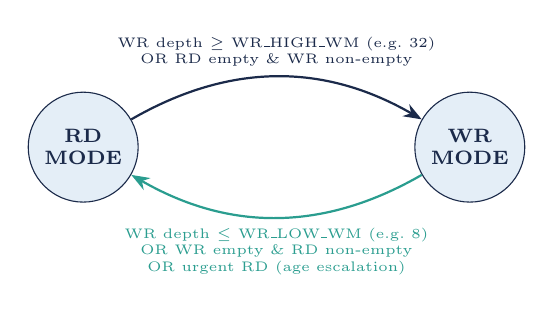
\begin{tikzpicture}[node distance=1.2cm and 2.0cm]
  \node[st] (rdm) {RD\\MODE};
  \node[st,right=3.5cm of rdm] (wrm) {WR\\MODE};

  \draw[arr,bend left=30] (rdm) to
    node[above,font=\tiny,align=center]
    {WR depth $\geq$ WR\_HIGH\_WM (e.g.\ 32)\\
     OR RD empty \& WR non-empty} (wrm);

  \draw[tarr,bend left=30] (wrm) to
    node[below,font=\tiny,align=center]
    {WR depth $\leq$ WR\_LOW\_WM (e.g.\ 8)\\
     OR WR empty \& RD non-empty\\
     OR urgent RD (age escalation)} (rdm);
\end{tikzpicture}
\end{center}

Hysteresis gap (HIGH $-$ LOW $= 24$ entries) prevents mode thrashing.

\subsection{REF Credit Tracker}

\[
\texttt{REF\_credits} \mathrel{+}= 1 \quad \text{every } t_{REFI}
\qquad
\texttt{REF\_credits} \mathrel{-}= 1 \quad \text{on REF issued}
\]
\[
\texttt{ref\_urgent} = (\texttt{REF\_credits} \geq 8)
\;\vee\;
(\Delta t_{\text{since last REF}} > t_{REFI\_max})
\]

JEDEC allows max 8 postponed refreshes (tREFI $\times$ 8 burst window).
When \texttt{ref\_urgent} asserts: arbitration outputs REF unconditionally.

\subsection{Arbitration Output Signals}

\begin{center}
\begin{tabularx}{0.85\linewidth}{@{} l l X @{}}
\toprule
\THead{Signal} & \THead{Width} & \THead{Description} \\
\midrule
\RA \texttt{arb\_winner} & 3b &
  \texttt{RD/WR/REF/ZQ/MRR/NOP} \\
\RB \texttt{pool\_ptr} & $\lceil\log_2 N\rceil$b &
  Index into winning pool (oldest or age-promoted entry) \\
\RA \texttt{mode\_state} & 1b &
  Current RD\_MODE (0) / WR\_MODE (1); fed back to watermark \\
\RB \texttt{ref\_urgent} & 1b &
  Hard-stall flag to all downstream logic \\
\bottomrule
\end{tabularx}
\end{center}

%%%%%%%%%%%%%%%%%%%%%%%%%%%%%%%%%%%%%%%%%%%%%%%%%%%%%%%%%%%%%%%%%%%%%%%%%%%%
\section{Command Selector}
%%%%%%%%%%%%%%%%%%%%%%%%%%%%%%%%%%%%%%%%%%%%%%%%%%%%%%%%%%%%%%%%%%%%%%%%%%%%

\subsection{Function}

Takes arbitration's winner class → applies \textbf{all DRAM timing constraints}
→ emits legal command sequence: \texttt{\{cmd\_type, rank, BG, bank, row, col\}}.
This is the most constraint-heavy block in the MC.

\subsection{Internal Block Diagram}

\begin{center}
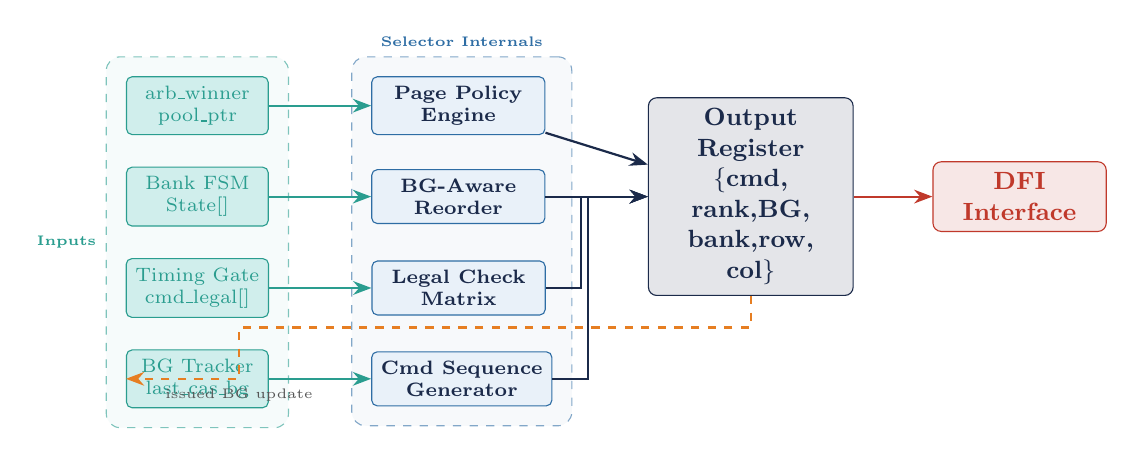
\begin{tikzpicture}[node distance=0.55cm and 1.0cm]

  %% ── left inputs ──────────────────────────────────────────────────────────
  \node[pool] (arbin)  {arb\_winner\\pool\_ptr};
  \node[pool,below=0.4cm of arbin] (bfsm) {Bank FSM\\State[]};
  \node[pool,below=0.4cm of bfsm]  (tg)   {Timing Gate\\cmd\_legal[]};
  \node[pool,below=0.4cm of tg]    (bgt)  {BG Tracker\\last\_cas\_bg};

  %% ── submodules ───────────────────────────────────────────────────────────
  \node[submod,right=1.3cm of arbin]  (pp)   {Page Policy\\Engine};
  \node[submod,right=1.3cm of bfsm]   (bg)   {BG-Aware\\Reorder};
  \node[submod,right=1.3cm of tg]     (lc)   {Legal Check\\Matrix};
  \node[submod,right=1.3cm of bgt]    (seq)  {Cmd Sequence\\Generator};

  %% ── output ───────────────────────────────────────────────────────────────
  \node[blk=navy,right=1.3cm of bg,
        minimum width=2.6cm,minimum height=2.4cm]
        (out2) {Output\\Register\\$\{$cmd,\\rank,BG,\\bank,row,\\col$\}$};

  %% ── arrows ───────────────────────────────────────────────────────────────
  \draw[tarr] (arbin) -- (pp);
  \draw[tarr] (bfsm)  -- (bg);
  \draw[tarr] (tg)    -- (lc);
  \draw[tarr] (bgt)   -- (seq);

  \draw[arr] (pp)  -- (out2);
  \draw[arr] (bg)  -- (out2);
  \draw[arr] (lc.east) -- ++(0.45,0) |- (out2.west);
  \draw[arr] (seq.east) -- ++(0.45,0) |- (out2.west);

  %% ── feedback BG tracker ─────────────────────────────────────────────────
  \draw[aarr,dashed] (out2.south) -- ++(0,-0.4)
    -- ++(-6.5,0) |- (bgt.west)
    node[midway,below,lbl]{issued BG update};

  %% ── to DFI ───────────────────────────────────────────────────────────────
  \node[blk=red,right=1.0cm of out2,minimum height=0.7cm,minimum width=2.2cm]
        (dfi) {DFI\\Interface};
  \draw[rarr] (out2) -- (dfi);

  %% ── group ────────────────────────────────────────────────────────────────
  \begin{scope}[on background layer]
    \node[grp=teal,fit=(arbin)(bfsm)(tg)(bgt),
          label={[font=\tiny\bfseries,color=teal]left:Inputs}]{};
    \node[grp=steel,fit=(pp)(bg)(lc)(seq),
          label={[font=\tiny\bfseries,color=steel]above:Selector Internals}]{};
  \end{scope}

\end{tikzpicture}
\end{center}

\subsection{Page Policy Engine}

\subsubsection{Open Page (Default)}

\begin{center}
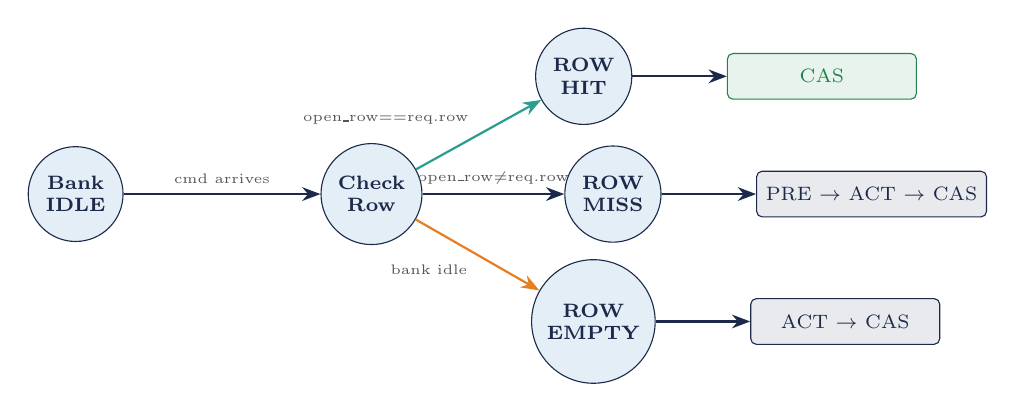
\begin{tikzpicture}[node distance=0.8cm and 1.6cm]
  \node[st] (idle) {Bank\\IDLE};
  \node[st,right=2.5cm of idle]  (act)  {Check\\Row};
  \node[st,above right=0.6cm and 1.8cm of act] (hit) {ROW\\HIT};
  \node[st,right=1.8cm of act]                 (mis) {ROW\\MISS};
  \node[st,below right=0.6cm and 1.8cm of act] (emp) {ROW\\EMPTY};

  \draw[arr] (idle) -- node[above,lbl]{cmd arrives} (act);
  \draw[tarr] (act) -- node[above left,lbl]{open\_row==req.row} (hit);
  \draw[arr]  (act) -- node[above,lbl]{open\_row$\neq$req.row} (mis);
  \draw[aarr] (act) -- node[below left,lbl]{bank idle} (emp);

  \node[sblk=grn,right=1.2cm of hit]  (cas1) {CAS};
  \node[sblk=navy,right=1.2cm of mis] (prac) {PRE $\to$ ACT $\to$ CAS};
  \node[sblk=navy,right=1.2cm of emp] (ac2)  {ACT $\to$ CAS};

  \draw[arr] (hit) -- (cas1);
  \draw[arr] (mis) -- (prac);
  \draw[arr] (emp) -- (ac2);
\end{tikzpicture}
\end{center}

\subsubsection{Policy Comparison}

\begin{center}
\begin{tabularx}{\linewidth}{@{} l X X X @{}}
\toprule
\THead{Policy} & \THead{Row Hit} & \THead{Row Miss} & \THead{Best For} \\
\midrule
\RA Open Page & CAS only & PRE+ACT+CAS & Sequential, high locality \\
\RB Closed Page & ACT+CAS & ACT+CAS & Random / streaming \\
\RA Adaptive & Hit-rate decides & Sliding window $N=256$ &
  Mixed workloads; auto-tunes \\
\bottomrule
\end{tabularx}
\end{center}

\textbf{Adaptive thresholds:} hit\_rate $>$ OPEN\_THR (e.g.\ 70\%) $\Rightarrow$ open;
hit\_rate $<$ CLOSE\_THR (e.g.\ 30\%) $\Rightarrow$ closed.

\subsection{Bank Group Aware Reordering}

DDR5 imposes large same-BG write penalties:
$t_{CCD\_L\_WR} = \max(32\,\text{nCK},\,20\,\text{ns})$
vs.\ $t_{CCD\_S} = 8\,\text{nCK}$ (diff BG).

Selector scans candidate queue for cross-BG entries to exploit the shorter gap:

\begin{center}
\begin{tabularx}{\linewidth}{@{} l l l @{}}
\toprule
\THead{Transition} & \THead{Same BG} & \THead{Diff BG} \\
\midrule
\RA RD$\to$RD & $t_{CCD\_L}=\max(8\,\text{nCK},5\,\text{ns})$ &
  $t_{CCD\_S}=8\,\text{nCK}$ \\
\RB WR$\to$WR & $t_{CCD\_L\_WR}=\max(32\,\text{nCK},20\,\text{ns})$ &
  $t_{CCD\_S\_WR}=8\,\text{nCK}$ \\
\RA WR$\to$WR (2nd not RMW) & $t_{CCD\_L\_WR2}=\max(16\,\text{nCK},10\,\text{ns})$ &
  $t_{CCD\_S}$ \\
\bottomrule
\end{tabularx}
\end{center}

Reordering is bounded by age limit to prevent starvation.

\subsection{Legal Check Matrix}

Full constraint vector checked per candidate before dispatch.
Any false bit $\Rightarrow$ NOP inserted that cycle.

\begin{center}
\begin{tabularx}{\linewidth}{@{} l l X @{}}
\toprule
\THead{Gate} & \THead{Timer Source} & \THead{Constraint Enforced} \\
\midrule
\RA \texttt{bank\_avail[b]} & Bank FSM state & Bank not in ACT/PRE transition \\
\RB \texttt{gate\_rcd[b]}   & ACT issue & $t_{RCD}$: ACT $\to$ first CAS \\
\RA \texttt{gate\_rp[b]}    & PRE issue & $t_{RP}$: PRE $\to$ ACT \\
\RB \texttt{gate\_ras[b]}   & ACT issue & $t_{RAS}$: ACT $\to$ PRE min \\
\RA \texttt{gate\_ccd\_l}   & Same BG CAS & $t_{CCD\_L}$ or $t_{CCD\_L\_WR}$ \\
\RB \texttt{gate\_ccd\_s}   & Diff BG CAS & $t_{CCD\_S}$ \\
\RA \texttt{gate\_rrd\_l}   & Same BG ACT & $t_{RRD\_L}$ \\
\RB \texttt{gate\_rrd\_s}   & Diff BG ACT & $t_{RRD\_S}$ \\
\RA \texttt{gate\_faw}      & Sliding ACT window & $\leq$4 ACTs within $t_{FAW}$ \\
\RB \texttt{gate\_wtr\_l}   & WR data end, same BG & $t_{WTR\_L}$: WR$\to$RD cmd \\
\RA \texttt{gate\_wtr\_s}   & WR data end, diff BG & $t_{WTR\_S}$: WR$\to$RD cmd \\
\RB \texttt{gate\_rtw}      & RD cmd & $t_{RTW}=t_{CL}+t_{BL/2}+2-t_{CWL}$ \\
\RA \texttt{gate\_rfc[r]}   & REF issue, per rank & $t_{RFC1}$: all cmds blocked \\
\RB \texttt{gate\_rfcpb[r][b]} & REFsb, per bank & $t_{RFCpb}$: same bank blocked \\
\RA \texttt{gate\_zqcs}     & ZQCS issue & All cmds blocked during ZQ \\
\RB \texttt{gate\_mrd}      & MRW issue & $t_{MRD}$: MRW to non-MR cmd \\
\RA \texttt{gate\_mod}      & MRW issue & $t_{MOD}$: MRW to normal ops \\
\bottomrule
\end{tabularx}
\end{center}

\subsection{Command Sequence Generator}

Outputs multi-beat sequences into a small 4-deep cmd FIFO.
During ACT/PRE wait cycles, \textbf{other banks may be serviced} (pipelining).

\begin{center}
\begin{tabularx}{\linewidth}{@{} l l @{}}
\toprule
\THead{Page Decision} & \THead{Emitted Sequence} \\
\midrule
\RA ROW HIT  & \texttt{CAS(RD/WR)} \\
\RB ROW MISS & \texttt{PRE} $\xrightarrow{t_{RP}}$ \texttt{ACT} $\xrightarrow{t_{RCD}}$ \texttt{CAS} \\
\RA ROW EMPTY & \texttt{ACT} $\xrightarrow{t_{RCD}}$ \texttt{CAS} \\
\RB REFab & \texttt{REFab} $\xrightarrow{t_{RFC1}}$ \texttt{NOP...} \\
\RA REFsb & \texttt{REFsb(bank)} $\xrightarrow{t_{RFCpb}}$ \texttt{NOP(that bank)}; others free \\
\RB ZQCS & \texttt{MPC ZQCALstart} $\xrightarrow{t_{ZQCAL}}$ \texttt{MPC ZQCALlatch}
  $\xrightarrow{t_{ZQLAT}}$ ready \\
\RA MRW & \texttt{MRW} $\xrightarrow{t_{MRD}}$ next cmd \\
\bottomrule
\end{tabularx}
\end{center}

\subsection{Output Signal Format}

\begin{center}
\begin{tabularx}{0.9\linewidth}{@{} l l X @{}}
\toprule
\THead{Field} & \THead{Width} & \THead{Description} \\
\midrule
\RA \texttt{cmd\_type} & 3b & ACT/RD/WR/PRE/REF/NOP/MRS/ZQCS \\
\RB \texttt{rank}      & 2b & Target rank \\
\RA \texttt{bank\_group} & 2--3b & BG[2:0] x4/x8; BG[1:0] x16 \\
\RB \texttt{bank}      & 2b & Bank within BG \\
\RA \texttt{row}       & 17b & Row address (ACT) \\
\RB \texttt{col}       & 11b & Column address (CAS) \\
\RA \texttt{ap}        & 1b & Auto-precharge flag \\
\RB \texttt{wr\_partial} & 1b & WR\_PARTIAL: triggers RMW path \\
\bottomrule
\end{tabularx}
\end{center}

%%%%%%%%%%%%%%%%%%%%%%%%%%%%%%%%%%%%%%%%%%%%%%%%%%%%%%%%%%%%%%%%%%%%%%%%%%%%
\section{Constraint Checklist}
%%%%%%%%%%%%%%%%%%%%%%%%%%%%%%%%%%%%%%%%%%%%%%%%%%%%%%%%%%%%%%%%%%%%%%%%%%%%

\subsection*{Legend: \cmark\ Supported \quad \xmark\ Not Supported / Deferred}

\subsubsection*{CAS-to-CAS Constraints}
\begin{center}
\begin{tabularx}{\linewidth}{@{} c l X @{}}
\toprule
\THead{} & \THead{Constraint} & \THead{Notes} \\
\midrule
\RA\cmark & $t_{CCD\_L}$ same BG RD$\to$RD &
  $\max(8\,\text{nCK},5\,\text{ns})$; BG tracker \\
\RB\cmark & $t_{CCD\_S}$ diff BG RD$\to$RD &
  8\,nCK; BG tracker \\
\RA\cmark & $t_{CCD\_L\_WR}$ same BG WR$\to$WR &
  $\max(32\,\text{nCK},20\,\text{ns})$ \\
\RB\cmark & $t_{CCD\_L\_WR2}$ same BG WR$\to$WR (2nd not RMW) &
  $\max(16\,\text{nCK},10\,\text{ns})$ \\
\RA\cmark & $t_{CCD\_S\_WR}$ diff BG WR$\to$WR &
  $= t_{CCD\_S} = 8\,\text{nCK}$ \\
\bottomrule
\end{tabularx}
\end{center}

\subsubsection*{ACT-to-ACT Constraints}
\begin{center}
\begin{tabularx}{\linewidth}{@{} c l X @{}}
\toprule
\THead{} & \THead{Constraint} & \THead{Notes} \\
\midrule
\RA\cmark & $t_{RRD\_L}$ same BG ACT$\to$ACT &
  $\max(8\,\text{nCK},5\,\text{ns})$ \\
\RB\cmark & $t_{RRD\_S}$ diff BG ACT$\to$ACT &
  8\,nCK \\
\RA\cmark & $t_{RRD\_L}(1\text{K})$ / $t_{RRD\_L}(2\text{K})$ page size variants &
  1KB and 2KB page differentiation \\
\RB\cmark & $t_{FAW}$ 4-ACT sliding window &
  4-entry shift register of ACT timestamps \\
\bottomrule
\end{tabularx}
\end{center}

\subsubsection*{ACT / PRE / Row Timing}
\begin{center}
\begin{tabularx}{\linewidth}{@{} c l X @{}}
\toprule
\THead{} & \THead{Constraint} & \THead{Notes} \\
\midrule
\RA\cmark & $t_{RCD}$ ACT$\to$CAS & Per-bank countdown \\
\RB\cmark & $t_{RP}$ PRE$\to$ACT & Per-bank countdown \\
\RA\cmark & $t_{RAS}$ min ACT$\to$PRE & Per-bank countdown \\
\RB\cmark & $t_{RC}$ = $t_{RAS}+t_{RP}$ ACT$\to$ACT same bank &
  Implicit from tRAS+tRP \\
\RA\cmark & $t_{RTP}$ RD$\to$PRE & WR burst end countdown \\
\RB\cmark & $t_{WR}$ WR$\to$PRE & CAS+$t_{WR}$ countdown \\
\RA\xmark & $t_{RAS}$ max (row open timeout) &
  Max $\approx9\times t_{REFI}$; force-PRE not implemented \\
\bottomrule
\end{tabularx}
\end{center}

\subsubsection*{Write/Read Turnaround}
\begin{center}
\begin{tabularx}{\linewidth}{@{} c l X @{}}
\toprule
\THead{} & \THead{Constraint} & \THead{Notes} \\
\midrule
\RA\cmark & $t_{WTR\_L}$ same BG WR$\to$RD &
  $t_{CWL}+t_{BL/2}+t_{WTR\_L}$ \\
\RB\cmark & $t_{WTR\_S}$ diff BG WR$\to$RD &
  $t_{CWL}+t_{BL/2}+t_{WTR\_S}$ \\
\RA\cmark & $t_{RTW}$ RD$\to$WR &
  $t_{CL}+t_{BL/2}+2-t_{CWL}$ \\
\bottomrule
\end{tabularx}
\end{center}

\subsubsection*{Refresh Constraints}
\begin{center}
\begin{tabularx}{\linewidth}{@{} c l X @{}}
\toprule
\THead{} & \THead{Constraint} & \THead{Notes} \\
\midrule
\RA\cmark & $t_{RFC1}$ REFab recovery & Per-rank block \\
\RB\cmark & $t_{RFCpb}$ REFsb per-bank recovery &
  Only that bank blocked; others free \\
\RA\cmark & $t_{REFI}$ interval tracking &
  7.8\,$\mu$s or 3.9\,$\mu$s ($>$85°C) \\
\RB\cmark & REF credit accumulation &
  Max 8; burst-of-8 support \\
\RA\cmark & \texttt{ref\_urgent} stall &
  Hard stall all RD/WR \\
\RB\cmark & $t_{REFI}$ derating 2$\times$ at $>$85°C via MR4 &
  MR4 polling; tREFI halved \\
\RA\xmark & Per-bank REF credit balance (REFsb full tracking) &
  Global credit only; per-bank balance not tracked \\
\RB\xmark & Automatic BA cycling for REFsb &
  BA00$\to$01$\to$10$\to$11 rotation not enforced \\
\RA\xmark & FGR 4$\times$ mode ($t_{REFI}/4$) &
  FGR 2$\times$ supported; 4$\times$ not \\
\RB\xmark & $t_{RFC2}$ FGR tRFC enforcement &
  FGR tRFC2 = 0.55$\times$tRFC1 not implemented \\
\bottomrule
\end{tabularx}
\end{center}

\subsubsection*{ZQ Calibration}
\begin{center}
\begin{tabularx}{\linewidth}{@{} c l X @{}}
\toprule
\THead{} & \THead{Constraint} & \THead{Notes} \\
\midrule
\RA\cmark & $t_{ZQCAL}$ ZQCAL start duration & \\
\RB\cmark & $t_{ZQLAT}$ ZQCAL latch wait & \\
\RA\cmark & $t_{ZQCS}$ periodic short cal interval & CSR-configurable \\
\RB\cmark & ZQCL stall during init & Init FSM handles \\
\bottomrule
\end{tabularx}
\end{center}

\subsubsection*{Mode Register}
\begin{center}
\begin{tabularx}{\linewidth}{@{} c l X @{}}
\toprule
\THead{} & \THead{Constraint} & \THead{Notes} \\
\midrule
\RA\cmark & $t_{MRD}$ MRW$\to$any non-MR & \\
\RB\cmark & $t_{MOD}$ MRW$\to$normal ops & \\
\RA\cmark & $t_{MRW}$ MRW$\to$MRW & \\
\RB\cmark & $t_{MRR}$ MRR$\to$next cmd & \\
\bottomrule
\end{tabularx}
\end{center}

\subsubsection*{DFI Latency / Pipelining}
\begin{center}
\begin{tabularx}{\linewidth}{@{} c l X @{}}
\toprule
\THead{} & \THead{Constraint} & \THead{Notes} \\
\midrule
\RA\cmark & \texttt{dfi\_t\_rddata\_en} &
  RD cmd $\to$ rddata\_en issued RL cycles ahead \\
\RB\cmark & \texttt{dfi\_t\_phy\_wrlat} &
  WR cmd $\to$ wrdata\_en issued WL cycles ahead \\
\RA\cmark & \texttt{dfi\_freq\_ratio} &
  1:1, 1:2, 1:4 nCK per DFI clk \\
\RB\xmark & CRC latency adder &
  Read CRC RL adder (MR8 OP[7]=1) not pipelined \\
\bottomrule
\end{tabularx}
\end{center}

\subsubsection*{Power / Self Refresh}
\begin{center}
\begin{tabularx}{\linewidth}{@{} c l X @{}}
\toprule
\THead{} & \THead{Constraint} & \THead{Notes} \\
\midrule
\RA\cmark & $t_{CKSRX}$ stable clock before SRX cmd & Init FSM + CKE logic \\
\RB\cmark & $t_{XS}$ SRX$\to$non-REF cmd & \\
\RA\cmark & $t_{XSR}$ SRX$\to$REF cmd & \\
\RB\xmark & MPSM entry/exit sequence &
  All-banks-precharged prerequisite not enforced \\
\RA\xmark & Power-down entry/exit $t_{CKE}$ etc. &
  Dynamic power-down not supported \\
\bottomrule
\end{tabularx}
\end{center}

\subsubsection*{ODT}
\begin{center}
\begin{tabularx}{\linewidth}{@{} c l X @{}}
\toprule
\THead{} & \THead{Constraint} & \THead{Notes} \\
\midrule
\RA\cmark & $\text{ODTL}_{on} = WL-2$ & \\
\RB\cmark & $\text{ODTL}_{off} = WL+BL/2$ & \\
\RA\cmark & $t_{ADC}$ ODT transition & \\
\RB\xmark & Dynamic RTT switching (RTT\_NOM\_RD vs RTT\_NOM\_WR) &
  Static RTT programming only; no auto-RTT switch per cmd \\
\bottomrule
\end{tabularx}
\end{center}

\subsubsection*{Multi-Rank / 3DS}
\begin{center}
\begin{tabularx}{\linewidth}{@{} c l X @{}}
\toprule
\THead{} & \THead{Constraint} & \THead{Notes} \\
\midrule
\RA\cmark & Per-rank $t_{RFC}$ isolation & \\
\RB\cmark & $t_{RRD}$ across ranks & \\
\RA\cmark & Rank interleave during $t_{RFC}$ bubble & \\
\RB\cmark & CID[3:0] die tracking (3DS) & \\
\RA\cmark & $t_{CCD\_slr}$ / $t_{CCD\_dlr}$ (3DS same/diff logical rank) & \\
\bottomrule
\end{tabularx}
\end{center}

\subsubsection*{RFM / Rowhammer}
\begin{center}
\begin{tabularx}{\linewidth}{@{} c l X @{}}
\toprule
\THead{} & \THead{Constraint} & \THead{Notes} \\
\midrule
\RA\xmark & RAA counter per bank &
  Rolling Accumulated ACT tracking not implemented \\
\RB\xmark & RAAIMT threshold monitoring &
  MR58 read \& comparison not implemented \\
\RA\xmark & RFMab command injection &
  No RFM command emitter \\
\RB\xmark & RFMsb command injection & \\
\RA\xmark & ALERT\_n RFM decode & \\
\bottomrule
\end{tabularx}
\end{center}

\subsubsection*{Training / Calibration (Scheduled)}
\begin{center}
\begin{tabularx}{\linewidth}{@{} c l X @{}}
\toprule
\THead{} & \THead{Constraint} & \THead{Notes} \\
\midrule
\RA\xmark & DQS oscillator start/stop scheduling &
  tDQS2DQ re-cal trigger not in MC \\
\RB\xmark & Periodic VREF sweep re-training &
  Post-init re-training not scheduled \\
\RA\xmark & CA parity retry scheduling &
  ALERT\_n decode + retransmit not implemented \\
\bottomrule
\end{tabularx}
\end{center}

\subsubsection*{Advanced / Optional Features}
\begin{center}
\begin{tabularx}{\linewidth}{@{} c l X @{}}
\toprule
\THead{} & \THead{Constraint} & \THead{Notes} \\
\midrule
\RA\xmark & $t_{RASmax}$ row open timeout &
  Force-PRE if row open $>9\times t_{REFI}$ \\
\RB\xmark & BL32 timing adjustments &
  $t_{CCD}$/$t_{WTR}$ extended by $BL/2=16$ nCK \\
\RA\xmark & $t_{CCD\_L\_WR2}$ vs $t_{CCD\_L\_WR}$ auto-select &
  RMW detection (WR\_PARTIAL flag) not wired to timer select \\
\RB\xmark & 2N mode CA pipeline re-timing &
  CS/CA setup/hold extension not enforced \\
\RA\xmark & Write Pattern command (WRP) scheduling & \\
\RB\xmark & PPR sequence scheduling &
  Guard key + hPPR/sPPR flow \\
\RA\xmark & ECS scrub address walking &
  MR14--MR21 scrub scheduling \\
\RB\xmark & Loopback / CT mode scheduling & \\
\RA\xmark & Per-parameter temperature derating table &
  Full JEDEC derating beyond 2$\times$ tREFI \\
\bottomrule
\end{tabularx}
\end{center}

\subsection{Summary Count}

\begin{center}
\begin{tabularx}{0.55\linewidth}{@{} l r @{}}
\toprule
\THead{Category} & \THead{Count} \\
\midrule
\RA \cmark\ Constraints Handled & \textbf{51} \\
\RB \xmark\ Not Supported / Deferred & \textbf{27} \\
\RA Total & \textbf{78} \\
\bottomrule
\end{tabularx}
\end{center}

\vspace{8pt}\hrule height 0.4pt\vspace{3pt}
{\scriptsize\color{dkgray}
Reference: JEDEC JESD79-5B (DDR5), MIPI DFI Spec v5.20.
Timing values device-specific; validate against datasheet for each speed bin.}

\end{document}
